\chapter{Sistema biometrico: elementi caratteristici}

\section{Struttura di un sistema biometrico}

\subsection{Struttura di un sistema biometrico (generale)}

\subsubsection{Fase di enrollment}

\begin{figure}[ht]
    \centering
    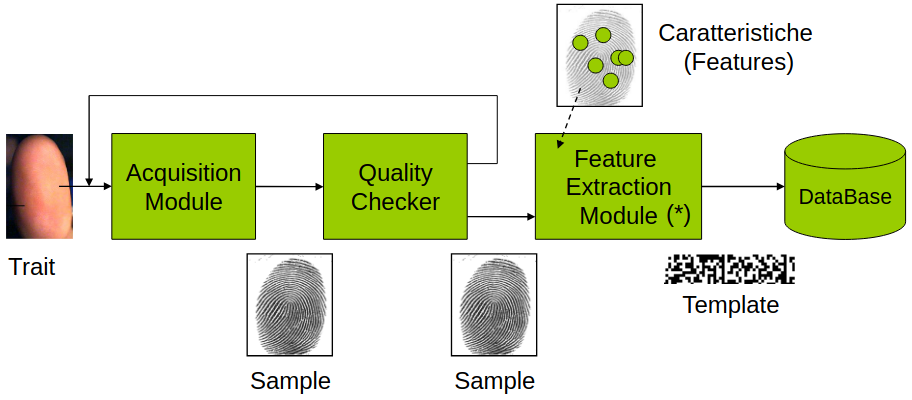
\includegraphics[width=0.95\linewidth]{chapters/images-chap2/enrollment-gen.png}
    \caption{Enrollment: (template) --$>$ DB}
    \label{fig:enroll-gen}
\end{figure}

\begin{figure}[ht]
    \centering
    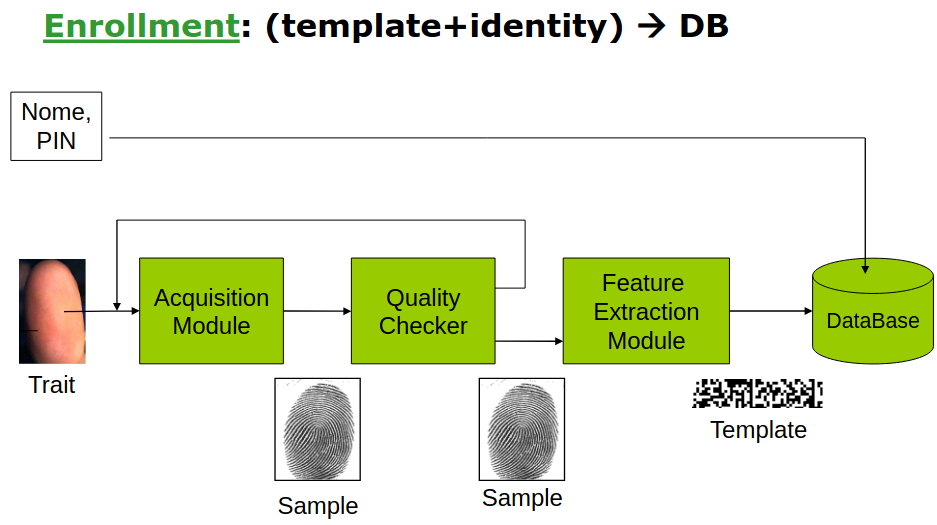
\includegraphics[width=0.95\linewidth]{chapters/images-chap2/enrollment-gen-id.png}
    \caption{(template + identity) --$>$ DB}
    \label{fig:enroll-gen-id}
\end{figure}

\newpage

\subsubsection{Verification usando un DB}

\begin{figure}[ht]
    \centering
    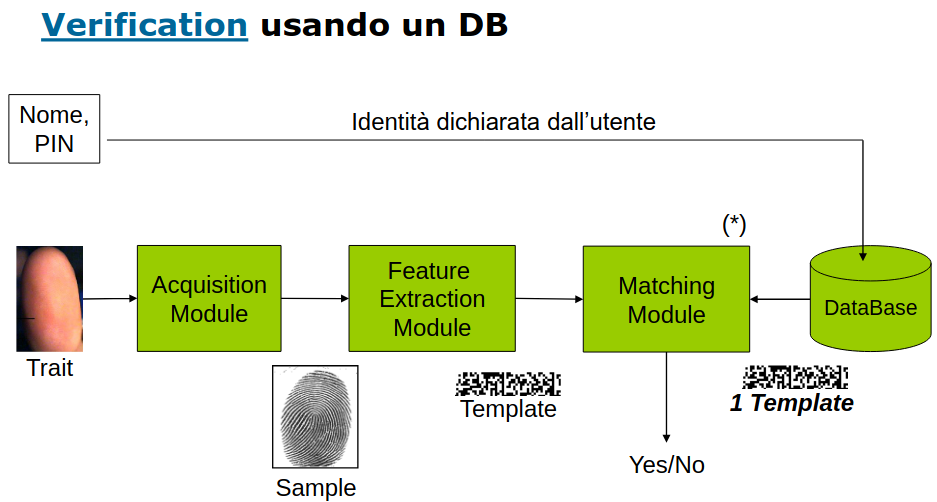
\includegraphics[width=0.95\linewidth]{chapters/images-chap2/verification-gen.png}
    \caption{Verification usando un DB}
    \label{fig:verification-gen}
\end{figure}

\newpage
\subsubsection{Identification}

\begin{figure}[ht]
    \centering
    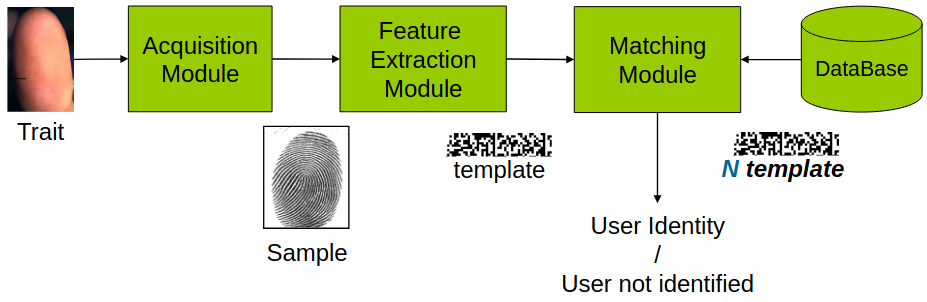
\includegraphics[width=0.95\linewidth]{chapters/images-chap2/identification-gen.png}
    \caption{Identification}
    \label{fig:id-gen}
\end{figure}

\subsection{Struttura per documenti biometrici}

\subsubsection{Fase di enrollment}

\begin{figure}[ht]
    \centering
    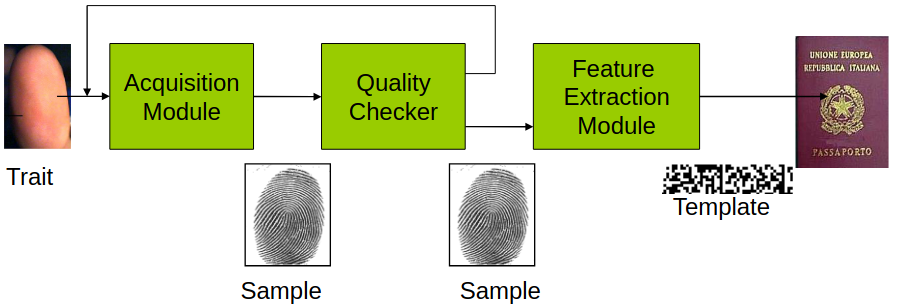
\includegraphics[width=0.95\linewidth]{chapters/images-chap2/enroll-doc.png}
    \caption{(template) --$>$ Documento}
    \label{fig:enroll-doc}
\end{figure}

\newpage
\subsubsection{Verification (con documento biometrico)}

\begin{figure}[ht]
    \centering
    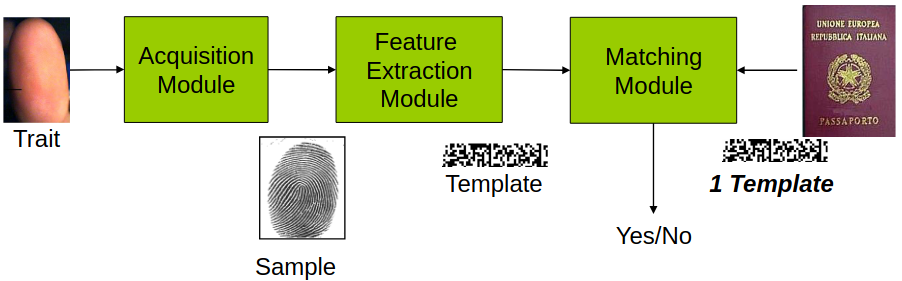
\includegraphics[width=0.95\linewidth]{chapters/images-chap2/verification-doc.png}
    \caption{Verification con documento biometrico}
    \label{fig:enter-label}
\end{figure}

\subsection{Struttura dei sistemi multimodali}

\begin{figure}[ht]
    \centering
    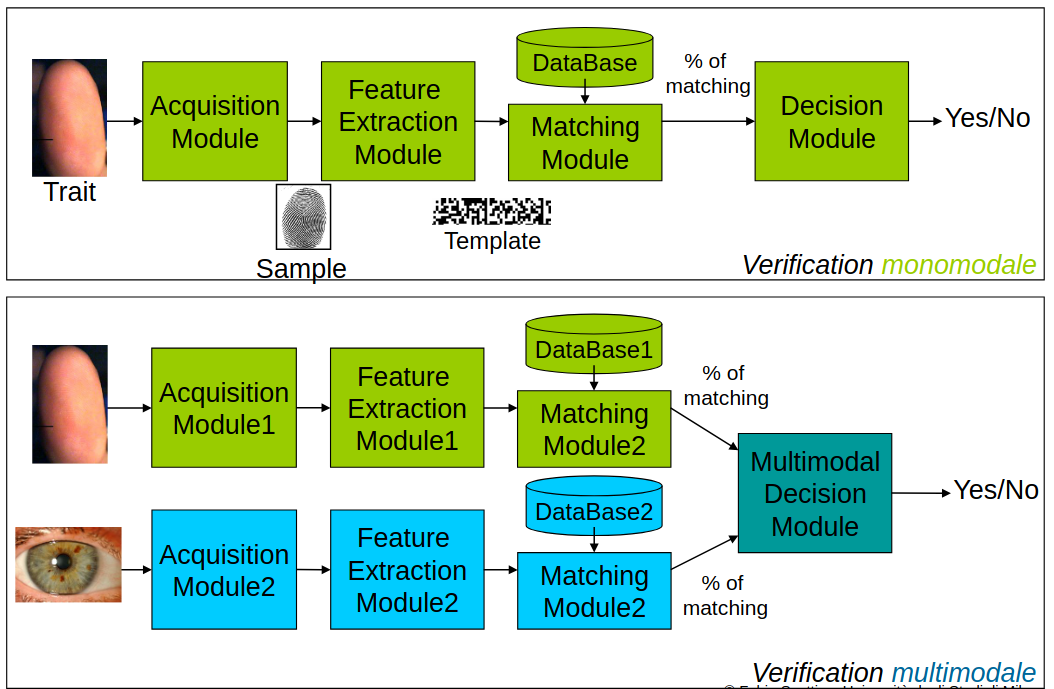
\includegraphics[width=0.95\linewidth]{chapters/images-chap2/multimodali.png}
    \caption{Confronto tra la struttura di un sistema monomodale e multimodale}
    \label{fig:multimodal}
\end{figure}

\subsection{Struttura dei sistemi biometrici distribuiti}

Il termine “distribuito” si riferisce ad un sistema biometrico quando i moduli componenti sono separati e collegati in rete.
Piuttosto raro quando si parla di sistemi di autenticazione; è invece comune quando si parla di sistemi di identificazione di grosse dimensioni. 


Solitamente è il modulo dei database ad essere separato dai terminali.
\begin{figure}[ht]
    \centering
    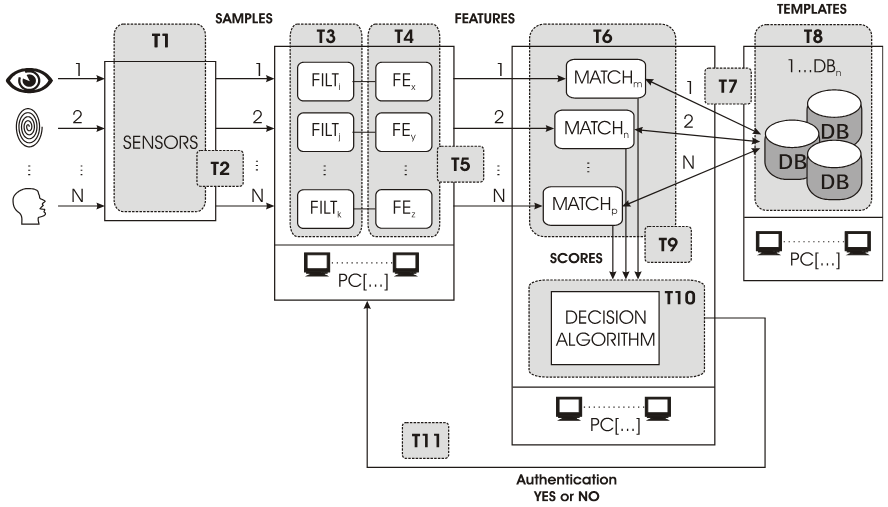
\includegraphics[width=0.95\linewidth]{chapters/images-chap2/distributed.png}
    \caption{Struttura di un sistema biometrico distribuito}
    \label{fig:distr}
\end{figure}

\subsection{Sistemi biometrici on card}
Il termine on card si riferisce al fatto che il template biometrico risiede su una smart card.

\section{Tratto biometrico: aspetti analitici}

\subsubsection{Variabilità intraclasse}

Si intende la variazione del \textbf{sample} o delle \textbf{feature} dello stesso individuo tra acquisizioni effettuate in istanti di tempo diversi.
Può essere dovuto a:
\begin{itemize}
    \item effetti casuali (rumore del dispositivo)
    \item varizioni dello sfondo
    \item variazioni del tratto (invecchiamento, posizione, espressioni, ecc.)
\end{itemize}

\subsubsection{Similitudine interclasse}

Particolare vicinanza dei \textbf{sample} o delle \textbf{feature} acquisiti da individui diversi.

\chapter{Regole Generali di Progettazione}

\section{Acquisizione del tratto}

Analizziamo i metodi per \textbf{progettare} ed eventualmente \textbf{migliorare} il modulo di acquisizione.

L'acquisizione di una informazione rilevante \textbf{è un processo critico} e non sempre adeguatamente studiato.

La cura nel processo di acquisizione \textbf{influenza pesantemente l'accuratezza} finale del sistema.

Il processo di acquisizione si divide in \textbf{due fasi:}
\begin{itemize}
    \item \textbf{Valutazione della qualità:} controllo automatico sulla correttezza dei dati in ingresso coerentemente alle successive elaborazioni
    \item \textbf{Segmentazione:} separazione dei dati in ingresso nell'oggetto di interesse (foreground) e nello sfondo/informazione non rilevante (background)
\end{itemize}

\subsubsection{Estrarre molte informazioni}

È buona prassi cercare di estrarre maggiori informazioni possibili per migliorare le performance del sistema biometrico.
\begin{itemize}
    \item \textbf{Acquisire anche il contesto} attorno al sample; permette di trovare meglio il vero volto per sottrazione di frame senza elaborazioni troppo complesse
    \item \textbf{Evitare sul nascere di fare cattive acquisizioni} per non dover richiedere il sample (ad esempio, controllare se il soggetto è in movimento o alla distanza corretta prima di elaborare il frame)
\end{itemize}

\subsection{Controllo della qualità}

Dopo l'acquisizione molti sistemi attuano un controllo automatico della qualità del tratto rilevato per evitare problemi di funzionamento.

I sistemi di controllo della qualità producono un \textbf{indice di qualità} del sample acquisito:
\begin{itemize}
    \item se l'indice di qualità è sufficientemente alto si prosegue
    \item altrimenti si torna ad acquisire un altro sample
\end{itemize}

Il concetto di base è semplice, ma la progettazione e realizzazione dell'indice di qualità non lo è; alcuni punti sono che:
\begin{itemize}
    \item non sempre esiste un \textbf{modello rigoroso e realistico} della misura in ingresso da usare per calcolare l'indice; ad esempio, se potessimo definire come dovrebbe essere un'immagine ottimale di un'impronta, potremmo esprime l'indice di qualità come la "distanza" dell'immagine in ingresso da quella ottima
    \item non sempre esistono \textbf{metriche rigorose e robuste} per misurare la distanza del sample in ingresso con il riferimento ottimale
\end{itemize}

\subsubsection{Signal/Image enhancement}
In alcuni casi non è possibile rifiutare un sample perché il suo indice di qualità è basso (ad esempio database giudiziari); in questo caso, il sistema cerca di estrarre le informazioni (foreground) dal rumore (background) in modo tale da far funzionare il resto della catena di moduli del sistema.

Solitamente questa fase è ad alta complessità computazionale. Può generare i cosidetti \textbf{artefatti}; ad esempio, data un'impronta rumorosa genere delle minuzie che non erano presenti nell'immagine originale.

\section{Rappresentazione}

Un'acquisizione di un sistema non elaborata, chiamata sample, è:
\begin{itemize}
    \item \textbf{non invariante} rispetto al momento dell'acquisizione
    \item \textbf{non discriminatoria} (sono tutte diverse)
\end{itemize}

In un sistema biometrico occorre \textbf{studiare come rappresentare al meglio l'informazione} per rispondere 
alla domanda: \textit{"Quale rappresentazione machine-readable cattura \textbf{completamente} l'informazione \textbf{invariante} e \textbf{discriminatoria} 
della misura in ingresso?}

Il problema della rappresentazione consiste nel determinare uno spazio di misura che sia:
\begin{itemize}
    \item \textbf{invariante} (meno variante) rispetto ad acquisizioni dello stesso individuo
    \item che si \textbf{differinzi massivamente} dalla acquisizioni di individui diversi
\end{itemize}
In altre parole, si può dire che la rappresentazione deve fornire:
\begin{itemize}
    \item \textbf{alta variabilità interclasse} (io diverso da tutti gli altri)
    \item \textbf{bassa variabilità intraclasse} (io simile a me stesso nei miei sample)
\end{itemize}

\begin{figure}[ht]
    \centering
    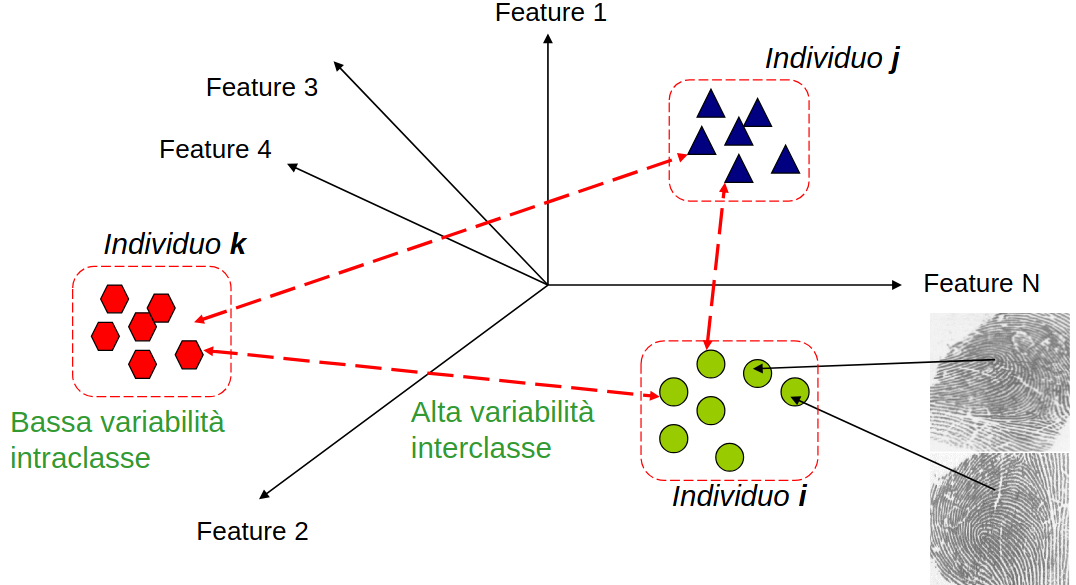
\includegraphics[width=1\linewidth]{chapters/images-chap2/rappresentazione.png}
    \caption{Visualizzazione del problema della
    rappresentazione in un spazio delle features
    N-dimensionale}
    \label{fig:rappr}
\end{figure}

Il problema della rappresentazione si suddivide in:
\begin{itemize}
    \item rappresentazione del sample
    \item estrazione delle caratteristiche
    \item rappresentazione del template
\end{itemize}

\subsection{Rappresentazione del sample}

Si riferisce alle caratteristiche tecniche del processo di acquisizione e memorizzazione del sample.
Varia a seconda del tratto biometrico, ci si riferisce a questi dati come \textbf{\textit{raw data}}.

\subsection{Estrazione di caratteristiche}

L'estrazione delle caratteristiche impatta sul modulo evidenziato
presente sia in fase di enrollment che di verification/identification.

\begin{figure}[ht]
    \centering
    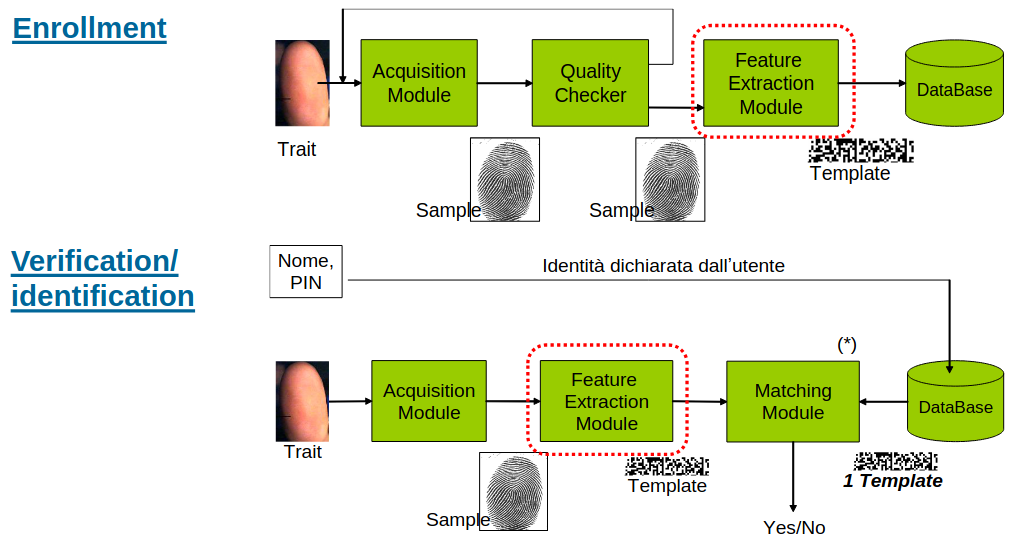
\includegraphics[width=1\linewidth]{chapters/images-chap2/estrazione.png}
    \caption{Impatto dell'estrazione delle caratterisiche}
\end{figure}

Avendo i dati raw provenienti dalle misurazioni occorre ora \textbf{estrarne la rappresentazione nello spazio delle caratteristiche.}
Questo non è mai un problema semplice, specialmente con dati rumorosi.

Può essere fatta in maniera manuale da un operatore oppure utilizzando un sistema automatico; \textbf{lo spazio delle 
caratteristiche di un sistema automatico tende ad essere diverso} da quello di un sistema con estrazione manuale.

\section{Matching}

Il matching impatta sul modulo evidenziato solo nella fase di verification\\/identification.

\begin{figure}[ht]
    \centering
    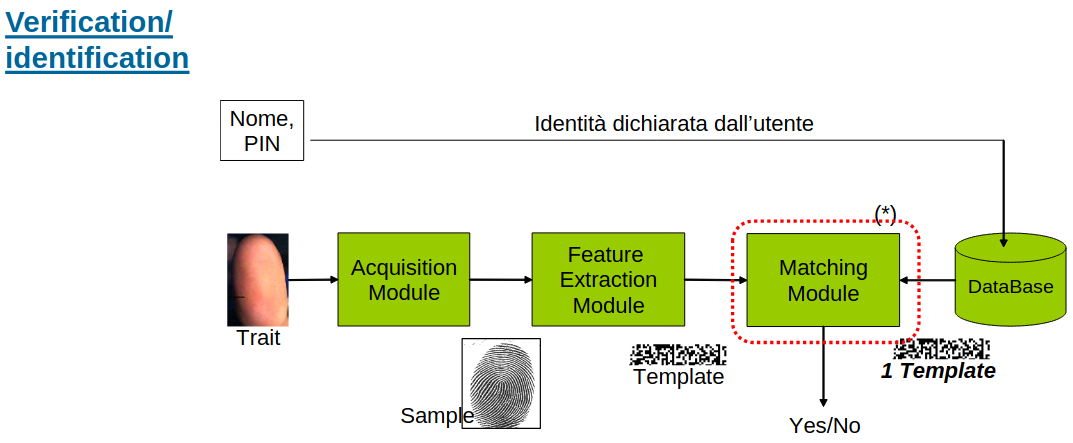
\includegraphics[width=1\linewidth]{chapters/images-chap2/matching.png}
    \caption{Impatto del matching}
\end{figure}

\section{Ricerca ed organizzazione dei DB biometrici}

\subsubsection{Scalabilità}

I sistemi che devono gestire una grande quantità di
identità dovrebbero essere in grado di operare
efficacemente quando il numero di utenti registrati nel DB
aumenta.

L'introduzione della biometria in un sistema di identificazione di grandi dimensioni produce dei vantaggi:
\begin{itemize}
    \item non soffrono del problema della produzione e del rinnovo dei documenti di identità
    \item sono competitivi in termini di costo e mantenimento
\end{itemize}

\subsection{Organizzazione del DB (indexing) e tasso di prenetazione nel DB}

L’obiettivo di gestire efficacemente la complessità delle
ricerche rispetto all’incremento del numero di template nel
DB del sistema può essere raggiunto solo con una attenta
organizzazione dei DB (indexing); un DB organizzato permette di non confrontare un
template in ingresso con tutti i template nel DB ma solo
con quelli contenuti in una partizione.

\begin{figure}[ht]
    \centering
    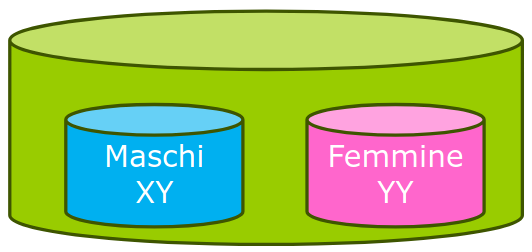
\includegraphics[width=0.75\linewidth]{chapters/images-chap2/indexing.png}
    \caption{Esempio di indexing}
\end{figure}

In generale si può definire il tasso di penetrazione come la
percentuale del database totale da esaminare in media per
ogni ricerca. Più basso è il tasso di penetrazione, più
efficiente è il sistema.

Tuttavia, per i sistemi biometrici serve fare un distinguo: 

\textit{\textbf{la proporzione attesa dei template da cercare su tutti i campioni di input secondo
la regola che la ricerca prosegue attraverso l'intera partizione, indipendentemente
dal fatto che venga trovata una corrispondenza o meno}}.

\subsection{Binning}

Per giovare delle partizioni del DB occorre disporre di un
\textbf{algoritmo automatico molto robusto} per la classificazione
dei template; quando il DB viene creato, i template vengono disposti nelle partizioni (\textbf{\textit{bins}}).

\begin{figure}[ht]
    \centering
    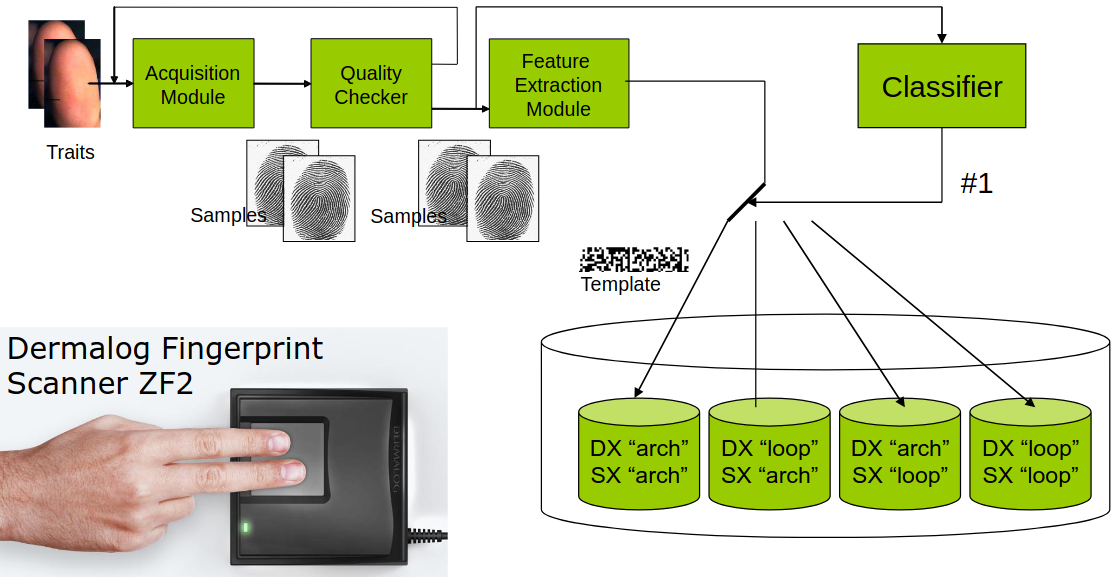
\includegraphics[width=1\linewidth]{chapters/images-chap2/binning.png}
    \caption{Esempio di suddivisioni in bins di un DB}
\end{figure}

\subsubsection{Calcolo del numero di bin ottimale}

Se ho \textbf{N} impronte disitnguibili (indice, medio...) tutte divisibili \textbf{M} tipi (arch, whorl, ...), allora 
numero migliore di bin è = \textbf{$M^N$}.

\subsubsection{Binning error}

I  problemi nascono quando un individuo presenta i propri
tratti biometrici al sistema e l’algoritmo di classificazione
del tratto sbaglia il bin (binning error); se l'indivduo era registrato nel DB, probabilmente non si avrà un match in quanto i template che matchano sono in un bin differente.

\newpage

\subsubsection{Calcolo del binning error}

Definiamo:

\textit{Binning error} = \textbf{Prob(}fare almeno 1 errore\textbf{)}

\textit{p} = \textbf{Prob(}sbagliare una classificazione\textbf{)} \\\\
Allora:

\textit{Binning error} = \textbf{Prob(}fare almeno 1 errore\textbf{)}

= 1 - \textbf{Prob(}0 errori\textbf{)}

= 1 - $(1-p)*(1-p)$

= 1 - $(p^2-2p+1)$

= $2p - p^2$ = 2p - \textit{molto poco (se p è piccola)}
\\
\\
Ne consegue che:

\textbf{Binning error} $\rightarrow$ \textbf{circa} $N*p$ \textbf{se si usano N impronte} se:

- \textit{p} è piccola (vero)

- classi distribuite (simile numero di impronte nei bin, vero)\\\\
Se si \textbf{abbassano il numero delle classi:}
\begin{itemize}
    \item \textbf{\textcolor{red}{Si alza il P.R. $\rightarrow$ si abbassa la qualità del P.R. ottenibile}}
    \item \textbf{\textcolor{green}{Si abbassa l'errore di classificazione}}
\end{itemize}




